\documentclass[a4paper, 9pt]{article}
\usepackage[utf8x]{inputenc}
\usepackage{graphicx}
\usepackage{geometry}
\usepackage{amsmath}
\usepackage{amssymb}
\usepackage{mathrsfs}

% OPENING
\title{SY 09 \\TP 1 :  Statistique descriptive, Analyse en composantes principales}
\author{Ricard Tatiana, Mehr Jean-Christophe}

\begin{document}

\maketitle

OBJECTIF DU TP 
\\* Les statistiques permettent depuis longtemps d’interpréter les données de manière objective et d’attribuer aux résultats un certain degré de confiance. Les outils de mesure et de récolte de données actuels nous permettent d’engranger un nombre colossal d’information. Il est donc devenu nécessaire d’être capable de traiter ces données et d’y appliquer les outils de visualisation adéquats.
Lors de ce TP nous allons tenter d’extraire des informations spécifiques à partir de différents jeux de données. En utilisant des outils appropriés et en appliquant un traitement préalable aux données si nécessaire.


\section{Statistique Descriptive}
\subsection{Donn\'ees babies}


Le jeu de données considéré
\textbf{ babies23.data}
est constitué de 1236 bébés décrits par 23 variables. Une fois le jeu de données chargé, nous sélectionnons 8 variables:\\
\\*-  5 quantitatives (le poids de naissance (birth weight), la dur\'ee de gestation, le nombre de grossesses pr\'ec\'edentes,
la taille de la m\`ere et le poids de la m\`ere)\\
\\* - 3 qualitatives (l'\^age de la m\`ere,
si la m\`ere fume ou non et le niveau d'\'education de la m\`ere).
\newline
% QUESTION
\newline\textbf{Q1) Quelle est la différence de poids entre les bébés nés de mères qui fumaient durant leur grossesse
et celles qui ne fumaient pas?}\\
Pour observer cette différence, nous pouvons étudier le résumé des valeurs du poids des b\'eb\'es en fonction du fait
du caractère fumeur de la mère :\\ \\
\begin{tabular}{|c|c|c|c|c|c|c|}
\hline
Min & 1st Qu. & Median & Mean & 3rd Qu. & Max \\
\hline
58.0 & 102.0 & 115.0 & 114.1 & 126.0 & 163.0 \\
\hline
\end{tabular}\\
\textit{R\'esum\'e des valeurs des b\'eb\'es n\'es d'une m\`ere fumeuse}\\ \\
\begin{tabular}{|c|c|c|c|c|c|c|}
\hline
Min & 1st Qu. & Median & Mean & 3rd Qu. & Max \\
\hline
55.0 & 113.0 & 123.0 & 123.0 & 134.0 & 176.0 \\
\hline
\end{tabular}\\
\textit{R\'esum\'e des valeurs des b\'eb\'es n\'es d'une m\`ere non fumeuse}\\ \\
\`Nous observons ainsi une diff\'erence entre les deux populations:\\
Suivant la moyenne et la m\'ediane des deux tableaux de donn\'ees, il semble que les enfants de mère fumeuse
aient un poids plus faible à la naissance que ceux d'une m\`ere non fumeuse.\\ \\
\newpage
Pour v\'erifier cette tendance, nous pouvons observer le graphique suivant :\\
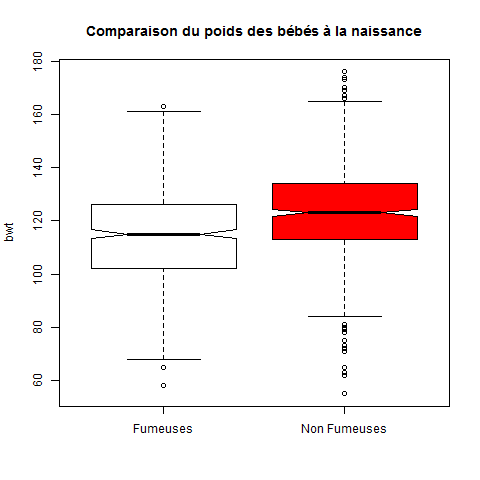
\includegraphics[height = 8cm, width = 8cm]{plots/boxplot_bwt_smoke.png}\\ \\
L'observation de ce boxplot nous permet de confirmer la tendance observ\'ee.
De plus, nous pouvons constater une pr\'esence plus importante de valeurs atypiques chez les m\`eres fumeuses.\\
Les intervalles de confiance pour les deux m\'edianes ne se chevauchent pas, nous pouvons
dire que la différence de poids est significative à 95\%.
\newpage
% QUESTION
\textbf{Q2) Est-ce qu’une mère qui fume durant sa grossesse est encline à avoir un temps de gestation plus
court qu’une mère qui ne fume pas?}\\
Pour répondre à cette question, nous étudions le résumé du temps de gestation en fonction du caractère fumeur de la mère :\\ \\
\begin{tabular}{|c|c|c|c|c|c|c|}
\hline
Min & 1st Qu. & Median & Mean & 3rd Qu. & Max\\
\hline
223.0 & 271.0 & 279.0 & 278.0 & 286.0 & 330.0\\
\hline
\end{tabular}\\
\textit{R\'esum\'e des valeurs du temps de gestation d'une m\`ere fumeuse}\\ \\
\begin{tabular}{|c|c|c|c|c|c|c|}
\hline
Min & 1st Qu. & Median & Mean & 3rd Qu. & Max\\
\hline
148.0 & 273.0 & 281.0 & 280.2 & 289.0 & 353.0\\
\hline
\end{tabular}\\
\textit{R\'esum\'e des valeurs du temps de gestation d'une m\`ere non fumeuse}\\ \\
Nous pouvons observer que les m\'edianes sont l\'eg\`erement diff\'erentes ce qui nous permet de dire que le fait de fumer peut conduire \`a
une modification sur la gestation mais il n'est pas possible d'établir clairement ce point avec les deux r\'esum\'es.\\ \\
Nous avons ensuite observ\'e les deux populations au moyen d'un boxplot :\\
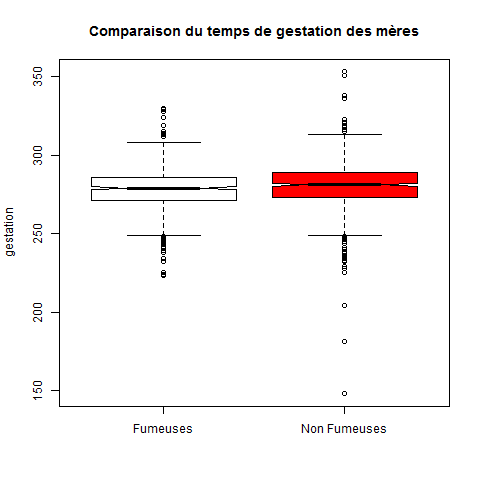
\includegraphics[height = 8cm, width = 8cm]{plots/boxplot_gestation_smoke.png}\\
On constate ici un nombre important de valeurs atypiques chez les femmes non-fumeuses.
Afin d'\'etudier ce boxplot au niveau des m\'edianes et des intervalles de confiance, nous choisissons de ne pas afficher ces valeurs afin d’avoir une meilleur représentativité de l’échantillon.
.\\
On observe ici un chevauchement des intervalles de confiance des m\'edianest, il n'est donc pas possible de conclure à une significativité de la différence de temps de gestation entre les mères fumeuse et non-fumeuses.
\newpage
% QUESTION
\textbf{Q3) Le niveau d’étude a-t-il une influence sur le fait que la mère soit fumeuse?}\\
Afin de r\'epondre \`a cette question, nous \'etudions dans un premier temps le tableau de contingence des donn\'ees :\\ \\
\begin{tabular}{|c|c|c|c|c|c|c|c|}
\hline
 & 0 & 1 & 2 & 3 & 4 & 5 & 7\\
\hline
M\`eres non fumeuses & 15 & 79 & 264 & 30 & 194 & 154 & 6 \\
\hline
M\`eres fumeuses & 4 & 102 & 176 & 33 & 102 & 65 & 1 \\
\hline
\end{tabular}\\
\\Le tableau de contingence nous permets de supposer un grand écart d’effectif entre le nombre de mère fumeuse et non fumeuse sur les niveaux d'étude 2, 4 et 5 (niveaux d’étude les plus représentés).
\\
Nous choisissons ensuite d’observer les deux populations de m\`eres au moyen d'un barplot :\\
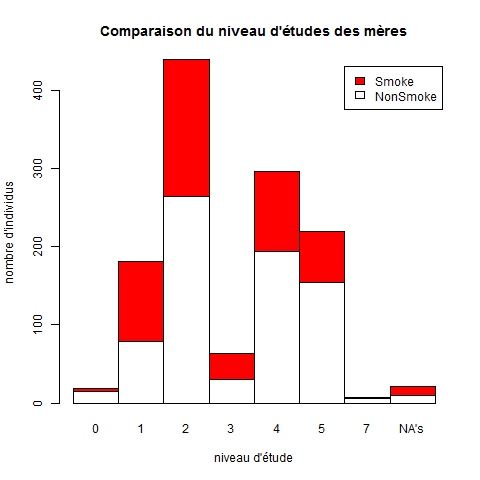
\includegraphics[height = 8cm, width = 8cm]{plots/barplot_etude_smoke.png}\\
Ce barplot illustre le tableau de contingence et fait apparaître visuellement que pour les niveaux d'\'etude 2, 4 et 5, il y a une plus grand proportions de
m\`eres non fumeuses alors quand le cas du niveau d'\'etude 1, Cette tendance est inversée.\\
En comparant nos résultats à l'\'etude pr\'esent\'ee,il est confirmé que les femmes non fumeuses ont tendance à avoir des bébés de poids plus élevé que les fumeuses.\\
L’étude évoque également l’absence de lien entre le temps de gestation et le caractère fumeur, ce qui explique que nous n’ayons pas pu déterminer de différence significative pour ce critère.
Concernant la relation entre le niveau d'\'etude et le tabagisme, nous remarquons à la rédaction de ce rapport qu’il aurait fallu effectuer la même étude en ramenant chacune des valeurs à un pourcentage. En effet, ici le nombre de femme non fumeuse évalué est de 742 alors que le nombre de femme fumeuse est inférieur à 500. Il est donc normal d’observer un nombre inférieur de femme fumeuse dans chaque catégorie d’étude. En prenant en compte ce fait, il semble tout de même que la proportion de femme fumeuse ayant un niveau d’étude supérieur à 4 est plus élevé.
\newpage
\subsection{Données crabs}


Le jeu de données considéré, disponible dans la bibliothèque de fonctions MASS, est constitué de 200 crabes décrits par huit variables (trois variables qualitatives, et cinq quantitatives). \\
\newline
% QUESTION
\textbf{Q1)  Existe-t-il des différences de caractéristiques morphologiques selon l’espèce ou le sexe? Semble-t-il possible d’identifier
l’espèce ou le sexe d’un crabe à partir d’une ou plusieurs mesures de ces caractéristiques?}\\
Nous affichons les donn\'ees des crabes en fonction de l'esp\`ece et du sexe des crabes :\\
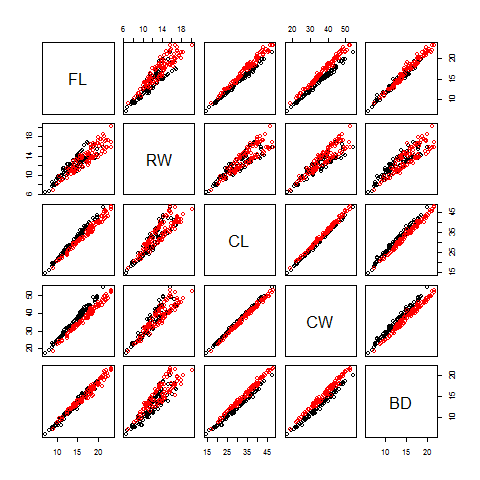
\includegraphics[height = 8cm, width = 8cm]{plots/plot_crabsquant_sp.png}
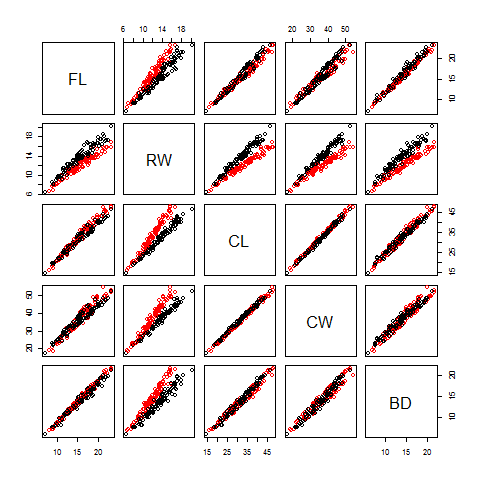
\includegraphics[height = 8cm, width = 8cm]{plots/plot_crabsquant_sex.png}\\
Ces deux graphiques nous montrent qu'il est difficile de d\'eterminer le sexe ou l'esp\`ece d'un crabe \`a partir des variables disponibles.\\
Afin de d\'eterminer l'existence de diff\'erences de caract\'eristiques morphologiques selon l'esp\`ece ou le sexe, nous comparons les donn\'ees
suivantes :\\
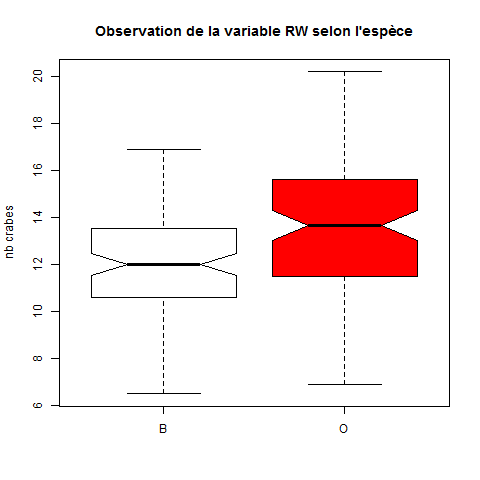
\includegraphics[height = 4cm, width = 3cm]{plots/boxplot_rw_espece.png}
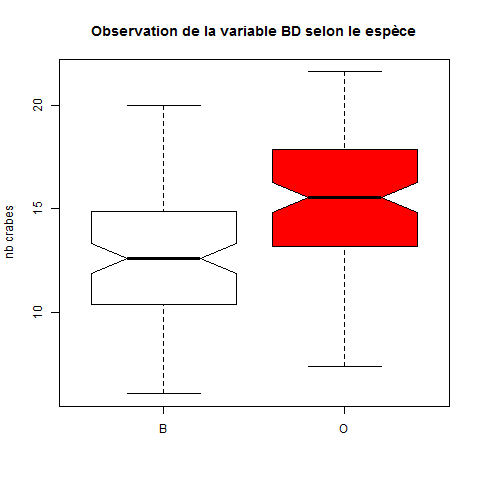
\includegraphics[height = 4cm, width = 3cm]{plots/boxplot_bd_espece.png}
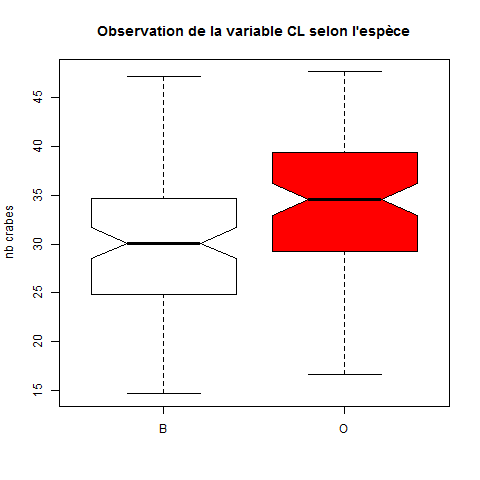
\includegraphics[height = 4cm, width = 3cm]{plots/boxplot_cl_espece.png}
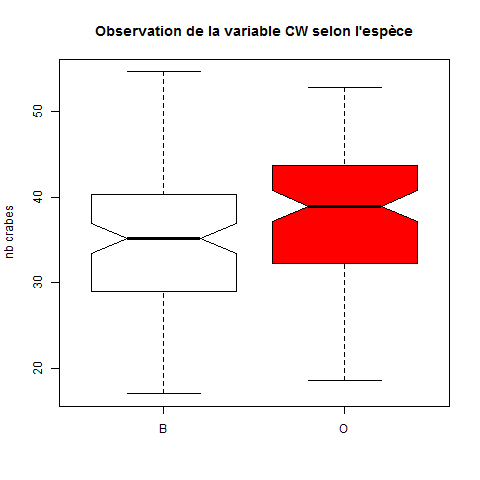
\includegraphics[height = 4cm, width = 3cm]{plots/boxplot_cw_espece.png}
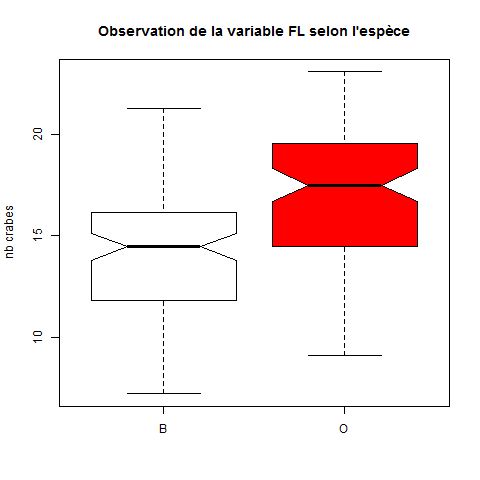
\includegraphics[height = 4cm, width = 3cm]{plots/boxplot_fl_espece.png}\\
En fonction des esp\`eces, nous pouvons voir que toutes les caract\'eristiques diff\`erent.
La dispersion des donn\'ees est par contre similaire pour chaque boxplot.\\ \\
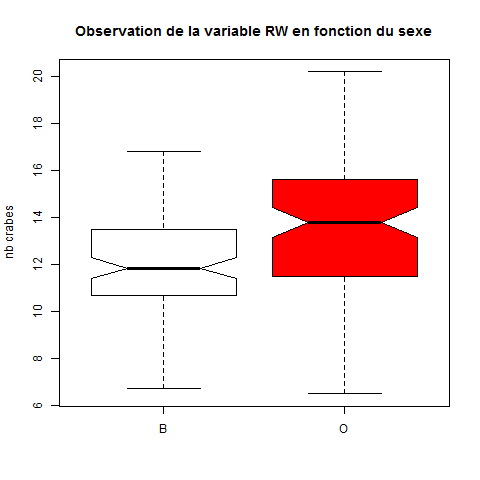
\includegraphics[height = 4cm, width = 3cm]{plots/boxplot_rw_sexe.png}
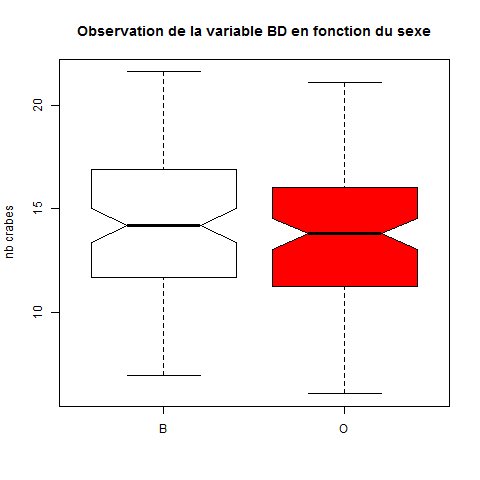
\includegraphics[height = 4cm, width = 3cm]{plots/boxplot_bd_sexe.png}
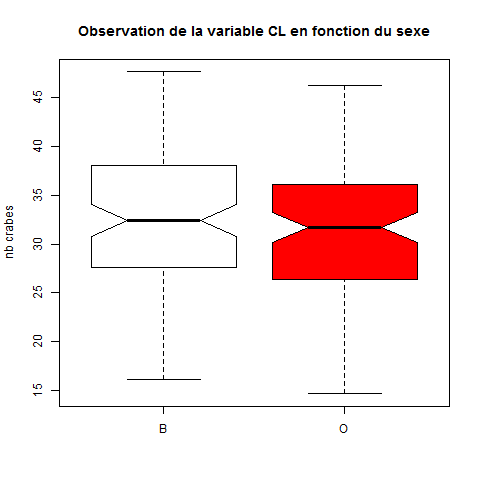
\includegraphics[height = 4cm, width = 3cm]{plots/boxplot_cl_sexe.png}
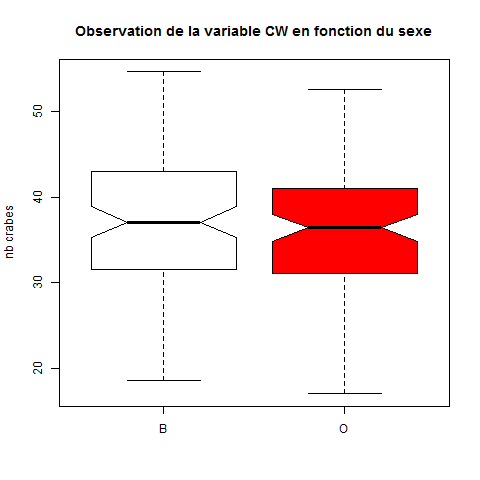
\includegraphics[height = 4cm, width = 3cm]{plots/boxplot_cw_sexe.png}
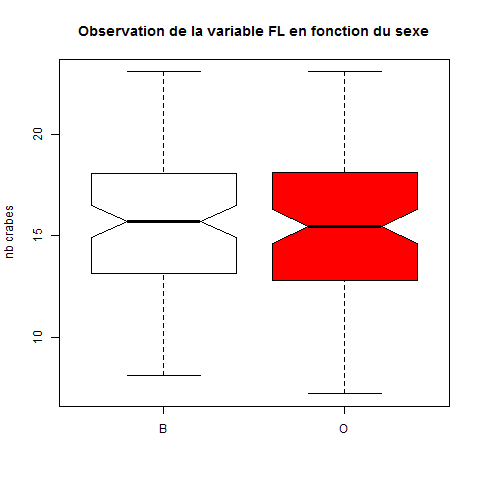
\includegraphics[height = 4cm, width = 3cm]{plots/boxplot_fl_sexe.png}\\
Par rapport au sexe des crabes, nous remarquons que toutes les caract\'eristiques (\`a part \textit{RW}) sont plut\^ot proches au vu
du chevauchement des intervalles de confiance et la dispersion des donn\'ees est environ la m\^eme pour les boxplots.\\ \\
Les crabes \textit{B} ont des valeurs plus \'elev\'ees pour toutes les variables quantitatives.\\ \\ \\ \\ \\
% QUESTION
\textbf{Q2) Quelle est vraisemblablement la cause de corrélation entre les variables ? Quel traitement est-il possible d’appliquer aux données pour
s’affranchir de ce phénomène? Quel traitement est-il possible d'appliquer aux donn\'ees pour s'affranchir de ce ph\'enom\`ene de corr\'elation ?}\\
Nous calculons dans un premier temps les coefficients de corrélation via la commande \textbf{cor} :\\ \\
\begin{tabular}{|c|c|c|c|c|c|c|}
\hline
 & FL & RW & CL & CW & BD\\
FL & 1.000 & 0.907 & 0.979 & 0.965 & 0.988\\
\hline
RW & 0.907 & 1.000 & 0.893 & 0.900 & 0.889\\
\hline
CL & 0.979 & 0.893 & 1.000 & 0.995 & 0.983\\
\hline
CW & 0.965 & 0.900 & 0.995 & 1.000 & 0.968\\
\hline
BD & 0.988 & 0.889 & 0.983 & 0.968 & 1.000\\
\hline
\end{tabular}\\


On a pu observer avec les différents outils appliqués une forte corrélation entre toutes les variables envisagées. Ce phénomène est dû à la nature des variables. En effet ce sont des variable morphologique liées à la taille du crabe.\\ \\


On observe que la variable la plus corr\'el\'ee est la variable \textit{CL} suite à la somme de ces corr\'elations.
Pour s'affranchir de ce ph\'enom\`ene de corr\'elation, il suffit de diviser les donn\'ees par cette variable, les variables restantes devraient ainsi être affranchies de l’influence de la taille générale de l’individu.


\newpage
\section{Analyse en composantes principales}
\subsection{Exercice th\'eorique}


Le but de cette partie est de comprendre l'ACP, une analyse permettant de traiter des donn\'ees multi-dimensionnelles d'un espace
large de variables en r\'eduisant celui-ci.
\[M =
\begin{pmatrix}
3 & 4 & 3\\
1 & 4 & 3\\
2 & 3 & 6\\
2 & 1 & 4
\end{pmatrix}\]\\
% QUESTION
\textbf{Calcul des axes factoriels de l'ACP du nuage d\'efini}\\
Pour obtenir les axes factoriels, on centre la matrice :
\[Mc =
\begin{pmatrix}
1 & 1 & -1\\
-1 & 1 & -1\\
0 & 0 & 2\\
0 & -2 & 0
\end{pmatrix}\]
puis on calcule la matrice de variance :
\[S = \frac{1}{n}*Mc*M = \frac{1}{4}*Mc*M =
\begin{pmatrix}
0.5 & 0 & 0\\
0 & 1.5 & -0.5\\
0 & -0.5 & 1.5
\end{pmatrix}\]
En diagonalisant cette matrice, nous obtenons les valeurs propres et les axes d'inertie suivants :\\ \\
\begin{tabular}{|c|c|c|c|}
\hline
 & $\lambda1$ & $\lambda2$ & $\lambda3$\\
\hline
valeurs propres & 2.0 & 1.0 & 0.5\\
\hline
\% axes d'inertie & 57.14 & 28.57 & 14.29\\
\hline
\% axes d'inertie cumul\'es & 57.14 & 85.71 & 100.0\\
\hline
\end{tabular}\\ \\
Nous pouvons remarquer que les deux premiers axes cumulent environ 86\% de l'information.
Donc nous pouvons repr\'esenter 86\% de l'information sur le plan factoriel d\'efini par les deux premiers axes.\\
Le calcul des composantes principales donne la matrice :\\
\[C =
\begin{pmatrix}
-1.41 & 0 & 1\\
-1.41 & 0 & -1\\
1.41 & 1.41 & 0\\
1.41 & -1.41 & 0
\end{pmatrix}\]
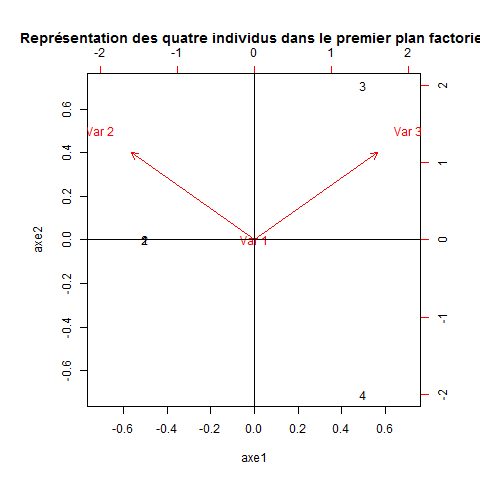
\includegraphics[height = 8cm, width = 8cm]{plots/plot_composantes_principales.png}\\
Sur ce graphique, nous pouvons observer que les deux premiers individus correspondent au m\^eme point dans le premier plan factoriel
et que la seule coordonn\'ee qui peut diff\'erencier ces deux points d\'epend du troisi\`eme axe factoriel.\\ \\
% QUESTION
\textbf{Traçage de la repr\'esentation des trois variables dans le premier plan factoriel}\\
On calcule les corr\'elations entre les variables pour avoir leurs coordonn\'ees sur le premier plan factoriel :\\
\[D = cor(Mc, C) =
\begin{pmatrix}
0 & 0 & 1\\
-0.816 & 0.577 & 0\\
-0.816 & 0.577 & 0
\end{pmatrix}\]
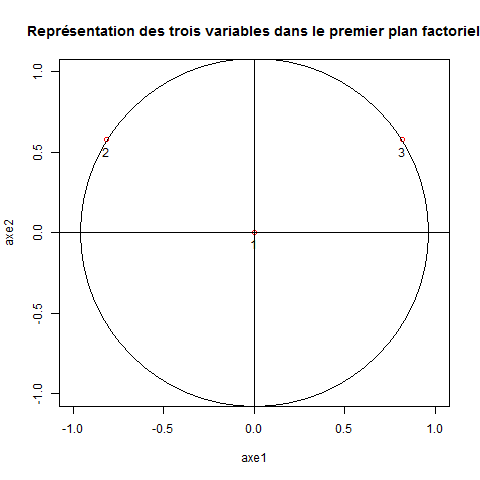
\includegraphics[height = 8cm, width = 8cm]{plots/plot_correlation.png}\\
% QUESTION
\textbf{Calcul de l'expression $\mathbf{\sum_{\alpha=0}^n c_{\alpha}.u'_{\alpha}}$ pour les valeurs \textit{k =} 1, 2 et 3}\\ \\
$k = 1 :
\begin{pmatrix}
0 & 1 & -1\\
0 & 1 & -1\\
0 & -1 & 1\\
0 & -1 & 1
\end{pmatrix}$,
$k = 2 :
\begin{pmatrix}
0 & 1 & -1\\
0 & 1 & -1\\
0 & 0 & 2\\
0 & -2 & 0
\end{pmatrix}$,
$k = 3 :
\begin{pmatrix}
1 & 1 & -1\\
-1 & 1 & -1\\
0 & 0 & 2\\
0 & -2 & 0
\end{pmatrix} = Mc$\newpage


\subsection{Utilisation des outils R}
% QUESTION
\textbf{Q1) Effectuer l’ACP du jeu de données notes étudiées en cours. Montrer
comment on peut retrouver tous les résultats alors obtenus (valeurs propres, axes principaux,
composantes principales, représentations graphiques)}\\
\\On calcule l'ACP avec l'instruction : \textit{acp = princomp(notes)}\\
On obtient les axes d'inertie et axes d'inertie cumul\'es avec l'instruction \textit{summary(acp)}\\
La matrice des composantes principales est contenue dans la variable \textit{acp\$scores}\\
Les vecteurs propres sont obtenue dans la variable \textit{acp\$loadings}\\
On établit le graphique de la repr\'esentation des individus :\\
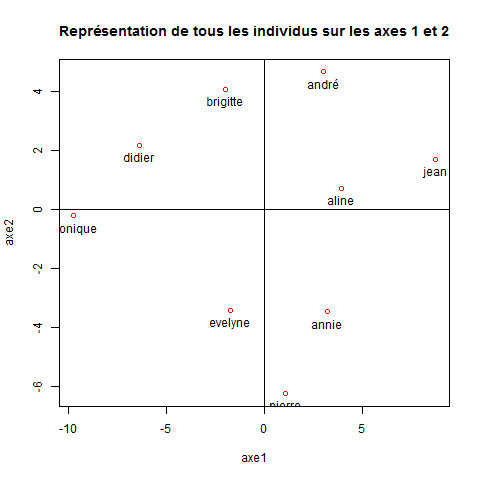
\includegraphics[height = 8cm, width = 8cm]{plots/plot_acp_notes.png}\\
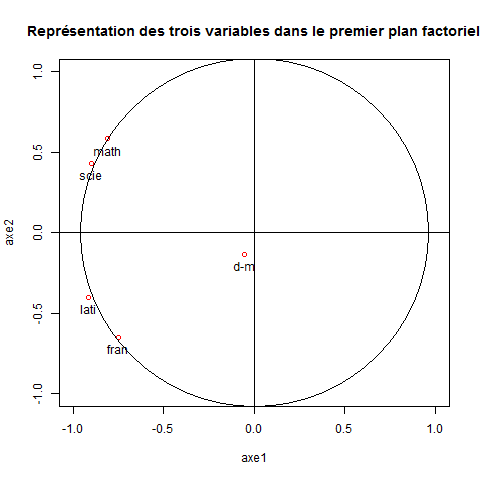
\includegraphics[height = 8cm, width = 8cm]{plots/plot_correlation_notes.png}
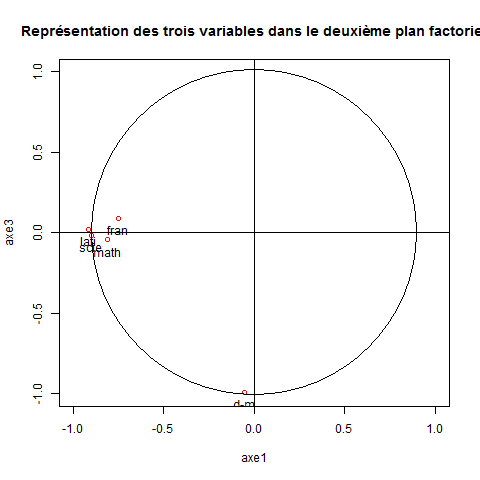
\includegraphics[height = 8cm, width = 8cm]{plots/plot_correlation_notes_2.png}\\ \\
% QUESTION
\textbf{Q2) Qu'affichent les fonctions \textit{plot} et \textit{biplot} ?}\\
La fonction \textit{princomp} r\'ealise l'ACP sur la matrice et nous retourne l'\'ecart-type pour la valeur \textit{sdev}.
La valeur \textit{loadings} nous permet d'avoir les axes factoriels, c'est-\`a-dire les vecteurs propres de la matrice de variance.
La valeur \textit{scores} nous donne la matrice des composantes principales.\\ \\
L'utilisation de la fonction \textit{plot} sur le r\'esultat de \textit{princomp} affiche les valeurs propres associ\'ees \`a chaque composante.\\
La fonction \textit{biplot} permet de projeter les individus et les variables sur un m\^eme plan.
Il est utile d'utiliser cette fonction pour \'evaluer graphiquement les corr\'elations entre les variables (par rapport \`a l'angle que forment
deux vecteurs). Deux variables sont ind\'ependantes si leur vecteur forment un angle de 90°.\\ \\
La fonction \textit{biplot.princomp} donne acc\`es \`a des options suppl\'ementaires par rapport \`a la fonction \textit{biplot}.
En argument nous avons l'objet de la classe \textit{princomp}, nous avons aussi la valeur \textit{choices} pour d\'efinir la taille des vecteurs
pour le plot. Nous avons aussi la valeur \textit{scale} pour obtenir une repr\'esentation standard des donn\'ees.
Pour finir, il y a la valeur \textit{pc.biplot} qui si elle est mise \`a TRUE, r\'ef\`ere \`a un plot avec des observations \'elargies par
la racine carr\'ee des n et des variables r\'eduites par cette racine carr\'ee.


\subsection{Traitement des donn\'ees Crabs}
% QUESTION
Comme dans l’exercice 1, on s’intéressera aux données crabs, et plus particulièrement aux descripteurs quantitatifs. On commence donc par charger les données et sélectionner les variables
quantitatives.\\


\textbf{Q1) Test de l’ACP sur crabsquant sans traitement préalable. Que constatez vous?}\\ \\
La repr\'esentation de l'ACP sans traitement pr\'ealable nous donne le graphique suivant :\\


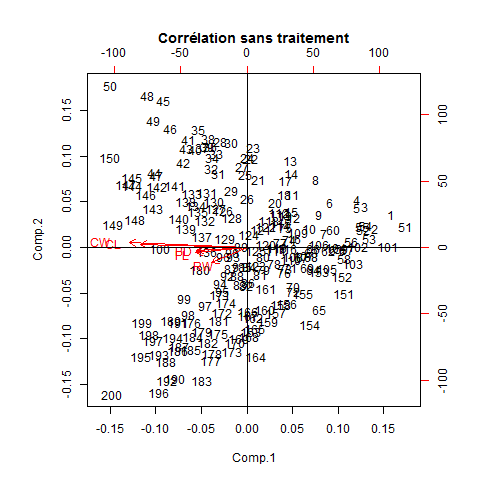
\includegraphics[height = 8cm, width = 8cm]{plots/biplot_acp2_crabs.png}
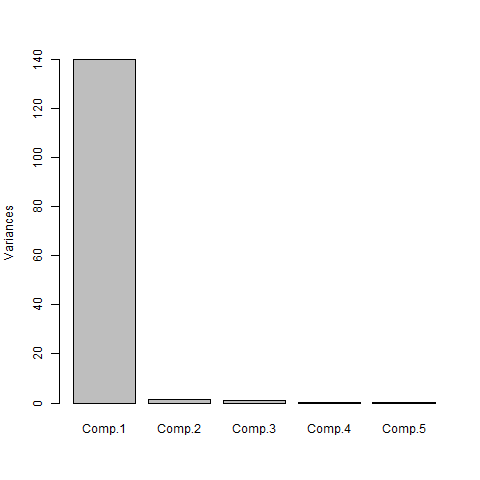
\includegraphics[height = 8cm, width = 8cm]{plots/plot_acp2_crabs.png}\\
Nous pouvons observer sur ce graphique la forte corr\'elation des variables comme confirmé dans les questions pr\'ec\'edentes.\\ \\
% QUESTION
\newpage
\textbf{Q2) Trouver une solution pour améliorer la qualité de votre représentation en termes de visualisation des différents groupes.}\\
\\Pour am\'eliorer la qualit\'e de la repr\'esentation en termes de visualisation, nous avons séparé la variable \textit{CL} et avons divisé le reste des varible par le vecteur ainsi obtenu. Ce qui nous permet de nous affranchir de l’influence de la taille général du crabe.
Nous avons ensuite refait une ACP et nous avons repr\'esent\'e les donn\'ees obtenues.\\
 \\ les variables ne sont ainsi plus corr\'el\'ees comme pr\'ec\'edemment ce qui nous donne les graphiques suivants :\\


\begin{figure}[h!]
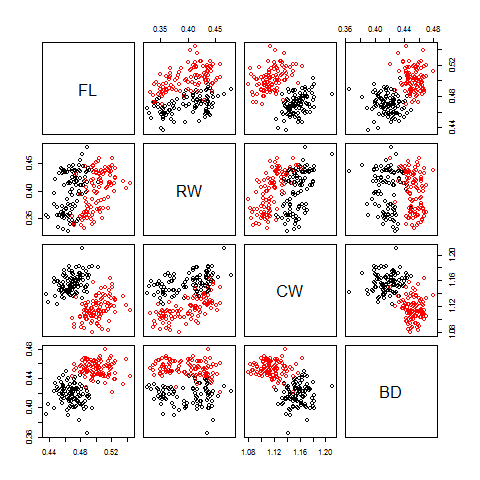
\includegraphics[height = 8cm, width = 8cm]{plots/plot_crabs_sp_2.png}
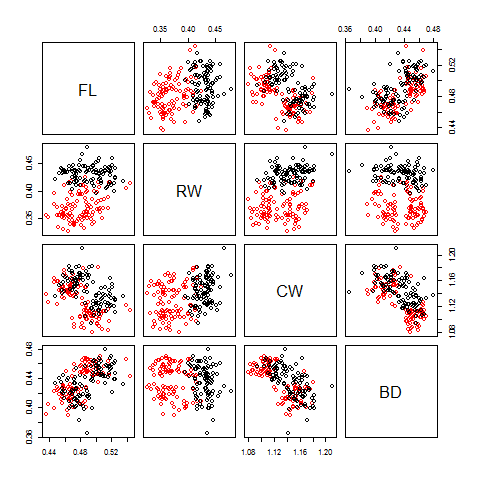
\includegraphics[height = 8cm, width = 8cm]{plots/plot_crabs_sex_2.png}
\caption{A gauche, graphique permettant de différencier les espèces. A droite, graphique permettant de différencier les sexes des crabes.}
\end{figure} 


\textbf{Conclusion :}\\
Effectuer un traitement préalable des données crabs nous a permis de mettre en évidence les différences significatives existantes pour chacun des critères en fonction du sexe et de l’espèce de l’individu. Cela peut par exemple permettre de déterminer ces deux caractéristiques (sexe et espèce) en fonction de la mesure des 4 paramètres de taille retenus. On comprend alors l’utilité d’un tel traitement et l’exploitation que l’on peut faire des données pour peu qu’on sache extraire l’information. 
\\ De manière général, ce TP nous a permis d’exploiter des jeux de données et d’en extraire des informations grâce à différents outils. Il a mis en évidence la complexité d’interpréter un grand nombre de données et la nécessité de parvenir à une représentation concluante et explicite.


\end{document}